% -*- coding: utf-8 -*-
% Beamer Presentation: LSMC Method for American Option Pricing
% Compiler: xelatex (twice)

\PassOptionsToPackage{table}{xcolor}
\documentclass[10pt,aspectratio=169]{beamer}

% --- Core Packages ---
\usepackage{amsmath,amssymb,amsthm,bm}
\usepackage{mathtools}
\usepackage{booktabs}
\usepackage{tikz}
\usepackage[most]{tcolorbox} 
\usetikzlibrary{arrows,positioning,shapes,calc}

% --- Metropolis Theme ---
\usetheme{metropolis}
\metroset{block=transparent}
\metroset{titleformat frame=regular}
\setbeamertemplate{navigation symbols}{}

% --- Colors ---
\definecolor{mathBlue}{RGB}{34,60,95}
\definecolor{mathGold}{RGB}{185,135,40}
\definecolor{boxBg}{RGB}{240,244,248}
\definecolor{errorColor}{RGB}{170,40,40}
\definecolor{itmGreen}{RGB}{46,139,87} % For ITM paths

% --- Highlighted Equation Boxes ---
\newcommand{\highlighteq}[1]{%
  \begin{center}
    \vspace{-0.1cm}
    \begin{tcolorbox}[
      colback=boxBg, colframe=mathGold, 
      boxrule=1.5pt, arc=2pt,
      top=4pt, bottom=4pt, left=4pt, right=4pt,
      width=0.95\linewidth, 
      halign=center, nobeforeafter
    ]
      $\displaystyle \fontsize{11}{14}\selectfont #1$
    \end{tcolorbox}
    \vspace{-0.1cm}
  \end{center}
}

\newcommand{\eqbox}[1]{%
  \begin{center}
    \vspace{-0.1cm}
    \begin{tcolorbox}[
      colback=white, colframe=mathBlue, 
      boxrule=1.0pt, arc=2pt,
      top=4pt, bottom=4pt, left=4pt, right=4pt,
      width=0.9\linewidth, 
      halign=center, nobeforeafter
    ]
      $\displaystyle \fontsize{10}{13}\selectfont #1$
    \end{tcolorbox}
    \vspace{-0.1cm}
  \end{center}
}

% --- TikZ Styles ---
\tikzset{
    block/.style={rectangle, draw, fill=gray!8, rounded corners,
                  minimum height=2.8em, text width=10em, text centered,
                  thick, draw=mathBlue, font=\small},
    blockSmall/.style={rectangle, draw, fill=gray!8, rounded corners,
                  minimum height=2.2em, text width=6em, text centered,
                  thick, draw=mathBlue, font=\small},
    line/.style={draw, ->, >=stealth, ultra thick, mathBlue},
    lineGold/.style={draw, ->, >=stealth, ultra thick, mathGold, dashed}
}

\newcommand{\R}{\mathbb{R}}
\newcommand{\Q}{\mathbb{Q}}
\newcommand{\F}{\mathcal{F}}
\newcommand{\E}{\mathbb{E}}
\newcommand{\argmin}{\operatorname{argmin}}
\newcommand{\de}{\mathrm{d}}

% ============================================
\begin{document}
% ============================================

% ============================================
% Slide 1: Title
% ============================================
\title{American Option Pricing via Least Squares Monte Carlo}
\subtitle{LSMC: Resolving Optimal Stopping Through $L^2$ Projection}
\author{\textbf{Your Name}}
\institute{School of Mathematical Sciences}
\date{July 2026}

\begin{frame}
  \titlepage
\end{frame}

% ============================================
% Slide 2: European vs American
% ============================================
\begin{frame}{From European to American: The Optimal Stopping Problem}

\textbf{Core distinction}: \textit{When} can the right to trade be exercised?
\vspace{0.1cm}
\\
\small \textcolor{gray!80}{Let $\Phi(S_t) = \max(K - S_t, 0)$ be the \textbf{Immediate Intrinsic Payoff} at time $t$.}

\vspace{0.3cm}
\begin{columns}[T] 
\begin{column}{0.48\textwidth}
\centering
\textbf{European Option} \\
\smallskip
\small Exercisable only at maturity $T$:
\highlighteq{
  V_E(0,S_0) = e^{-rT}\,\E^\Q\bigl[\Phi(S_T)\bigr]
}
\vspace{0.1cm}
\begin{itemize}
    \item Single expectation at $T$.
    \item Easy to simulate forward.
\end{itemize}
\end{column}
\begin{column}{0.48\textwidth}
\centering
\textbf{American Option} \\
\smallskip
\small Exercisable at any $\tau \in [0,T]$:
\highlighteq{
  V_A(0,S_0) = \sup_{\tau\in\mathcal{T}_{[0,T]}} \E^\Q\bigl[e^{-r\tau}\Phi(S_\tau)\bigr]
}
\vspace{0.1cm}
\begin{itemize}
    \item \textbf{Stochastic optimization} problem.
    \item Requires backward induction.
\end{itemize}
\end{column}
\end{columns}

\end{frame}

% ============================================
% Slide 3: The Core Dilemma (NEW LOGIC)
% ============================================
\begin{frame}{The Core Dilemma: Exercise vs. Hold}

To solve the optimal stopping problem, the holder faces a binary choice at each step $t$. The value $V_t$ follows the \textbf{Snell Envelope}:

\vspace{0.1cm}
\highlighteq{
  V_t = \max\bigl\{\underbrace{\Phi(S_t)}_{\text{Exercise}},\; \underbrace{C(t,S_t)}_{\text{Hold}}\bigr\}
}

\vspace{0.2cm}
\begin{itemize}
  \item \textbf{The Known (Easy)}: Immediate payoff $\Phi(S_t) = \max(K - S_t, 0)$.
  \item \textcolor{errorColor}{\textbf{The Unknown (Hard)}}: Continuation value $C(t,S_t)$. This is the expected discounted future payoff conditional on today's price.
\end{itemize}

\vspace{0.1cm}
\eqbox{
  C(t, S_t) = \E^\Q\bigl[\,e^{-r\Delta t}\,V_{t+\Delta t} \mid S_t\,\bigr]
}

\vspace{0.1cm}
\small \textbf{The Paradox}: Monte Carlo paths evolve \textit{forward} in time, but computing $C(t,S_t)$ requires information from the \textit{future (backward induction)}. How to bridge this?
\end{frame}

% ============================================
% Slide 4: The 8-Path Walk-Through (MOVED UP FOR INTUITION)
% ============================================
\begin{frame}{The Eureka Moment: The 8-Path Example}

\textbf{Setup}: American Put, 8 MC paths, 3 time steps, $K=1.10$. \\
At $t_2 = 2/3$, should we exercise? \textit{(Longstaff \& Schwartz use Cross-Sectional Regression)}

\vspace{0.2cm}
\begin{columns}[T]
\begin{column}{0.48\textwidth}
\begin{center}
\footnotesize
\renewcommand{\arraystretch}{1.1}
\setlength{\tabcolsep}{4pt}
\begin{tabular}{c|ccc|c}
\toprule
\textbf{Path} & $S_{t_1}$ & $S_{t_2}$ & $S_{T}$ & \textbf{ITM at $t_2$?} \\
\midrule
1 & 1.09 & \textcolor{itmGreen}{\textbf{1.08}} & 1.34 & \textcolor{itmGreen}{Yes} \\
2 & 1.16 & 1.26 & 1.54 & No \\
3 & 1.22 & \textcolor{itmGreen}{\textbf{1.07}} & 1.03 & \textcolor{itmGreen}{Yes} \\
4 & 0.93 & \textcolor{itmGreen}{\textbf{0.97}} & 0.92 & \textcolor{itmGreen}{Yes} \\
5 & 1.11 & 1.56 & 1.52 & No \\
6 & 0.76 & \textcolor{itmGreen}{\textbf{0.77}} & 0.90 & \textcolor{itmGreen}{Yes} \\
7 & 0.92 & \textcolor{itmGreen}{\textbf{0.84}} & 1.01 & \textcolor{itmGreen}{Yes} \\
8 & 0.88 & 1.22 & 1.34 & No \\
\bottomrule
\end{tabular}
\end{center}
\end{column}

\begin{column}{0.50\textwidth}
\footnotesize
\textbf{1. Regress} discounted future payoff $Y$ on $\{1, S, S^2\}$ \textbf{only} for the 5 ITM paths:
\vspace{-0.1cm}
\eqbox{
  \hat{C}(S) = -1.070 + 2.983\,S - 1.813\,S^2
}

\textbf{2. Decide} ($\text{Exercise if } \Phi > \hat{C}$):
\begin{center}
\renewcommand{\arraystretch}{1.1}
\setlength{\tabcolsep}{3pt} 
\begin{tabular}{c|c|c|c|c}
\toprule
\textbf{Path} & $S_{t_2}$ & $\Phi(S_{t_2})$ & $\hat{C}(t_2,S)$ & \textbf{Decision} \\
\midrule
1 & 1.08 & 0.02 & 0.039 & Hold \\
3 & 1.07 & 0.03 & 0.046 & Hold \\
\rowcolor{gray!20}4 & 0.97 & \textbf{0.13} & 0.118 & \alert{Exercise!} \\
\rowcolor{gray!20}6 & 0.77 & \textbf{0.33} & 0.152 & \alert{Exercise!} \\
\rowcolor{gray!20}7 & 0.84 & \textbf{0.26} & 0.157 & \alert{Exercise!} \\
\bottomrule
\end{tabular}
\end{center}
\end{column}
\end{columns}
\end{frame}

% ============================================
% Slide 5: Algorithm Overview (MOVED DOWN)
% ============================================
\begin{frame}{Formalizing the Intuition: The LSMC Algorithm}

\vspace{0.4cm}
\begin{center}
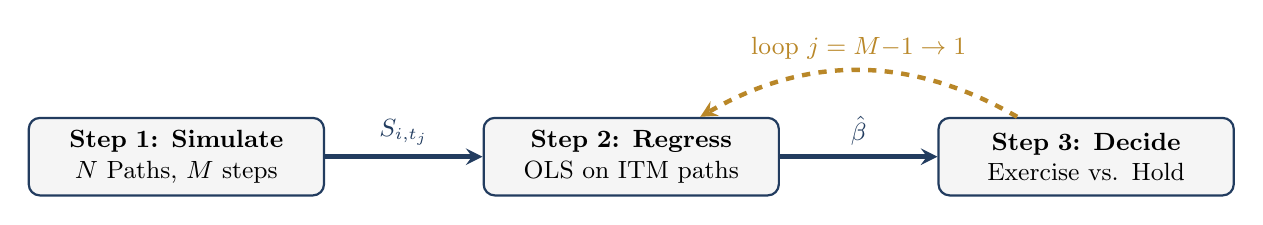
\begin{tikzpicture}[node distance=1.8cm, auto]
  \node [block] (MC) {\textbf{Step 1: Simulate}\\$N$ Paths, $M$ steps};
  \node [block, right=2.0cm of MC] (LS) {\textbf{Step 2: Regress}\\OLS on ITM paths};
  \node [block, right=2.0cm of LS] (DP) {\textbf{Step 3: Decide}\\Exercise vs. Hold};

  \draw[line] (MC) -- node[above,font=\small] {$S_{i,t_j}$} (LS);
  \draw[line] (LS) -- node[above,font=\small] {$\hat{\beta}$} (DP);
  \draw[lineGold] (DP) to [out=150, in=30] node[above,font=\small] {loop $j=M{-}1\to1$} (LS);
\end{tikzpicture}
\end{center}

\vspace{0.6cm}
\textbf{Core Methodology}:
\begin{itemize}
    \item Generate full paths forward to maturity.
    \item Step backward through time.
    \item Instead of nested simulations, use \textbf{cross-sectional regression} across all paths to estimate the conditional expectation function.
\end{itemize}
\end{frame}


% ============================================
% Slide 6: Step 2A (Math Details)
% ============================================
\begin{frame}{Step 2A: Estimating Continuation via $L^2$ Projection}

Recall our mathematical objective at each backward step $t_j$:
\eqbox{
  C(t_j, S_{t_j}) = \E^\Q\bigl[\,e^{-r\Delta t}\,V_{t_{j+1}} \mid S_{t_j}\,\bigr]
}

\textbf{Filter: Why only In-The-Money (ITM) paths?}
\begin{itemize}
    \item If $S_{t_j} > K$, immediate exercise yields $0$. The optimal choice is trivially to hold. Excluding Out-of-the-Money paths focuses the regression purely on the region where the exercise decision matters, vastly improving fit accuracy.
\end{itemize}

\vspace{0.1cm}
For ITM paths $\mathcal{I}_j$, regress realized cash flows $Y_{i} = e^{-r\Delta t} V_{i,t_{j+1}}$ onto basis $\{\psi_k\}$:
\highlighteq{
  \hat{\beta}_j = \argmin_{\beta\in\R^{d+1}}
  \sum_{i\in\mathcal{I}_j} \Bigl(Y_{i} - \sum_{k=0}^{d} \beta_k \psi_k(S_{i,t_j})\Bigr)^2
}

\end{frame}


% ============================================
% Slide 7: Step 2B
% ============================================
\begin{frame}{Step 2B: Exercise Decision and Cash Flow Update}

With $\hat{C}(t_j, S_{i,t_j}) = \sum_{k=0}^{d} \hat{\beta}_{j,k}\; \psi_k(S_{i,t_j})$ estimated, we compare:
\vspace{0.2cm}
\highlighteq{
  V_{i,t_j} =
  \begin{cases}
  \Phi(S_{i,t_j}) & \text{if } \Phi(S_{i,t_j}) > \hat{C}(t_j, S_{i,t_j}) \quad\text{(\textbf{Exercise})} \\[6pt]
  e^{-r\Delta t}\, V_{i,t_{j+1}} & \text{otherwise} \quad\text{(\textbf{Continue})}
  \end{cases}
}

\vspace{0.3cm}
\begin{itemize}
    \item \textbf{Loop}: Set $j \leftarrow j-1$ and repeat backward until reaching $t_1$.
    \item \textcolor{errorColor}{\textbf{Crucial Update Rule}}: Once a path is exercised at $t_j$, its future cash flows at $t_{j+1}, \dots, T$ are \textbf{set to zero} (since options can only be exercised once per path).
\end{itemize}
\end{frame}

% ============================================
% Slide 8: Step 3
% ============================================
\begin{frame}{Step 3: From Backward Induction to the Option Price}

Finally, at time $t_0 = 0$, we simply average the discounted cash flows from the very first optimal stopping time $\tau_i$ for each path:

\vspace{0.2cm}
\highlighteq{
  \hat{V}_0 = \frac{1}{N}\sum_{i=1}^{N} e^{-r\tau_i}\, \Phi(S_{i,\tau_i}) \equiv \frac{1}{N}\sum_{i=1}^{N} e^{-r\Delta t}\, V_{i,t_1}
}

\vspace{0.4cm}
\textbf{Convergence \& Error Decomposition (Clément et al., 2002):}
\begin{itemize}
    \item \textbf{Law of Large Numbers}: $\hat{V}_0 \to V_0$ as $N \to \infty$.
    \item \textbf{Total Error arises from}: 
    \begin{enumerate}
        \item Monte Carlo sampling error: $O(N^{-1/2})$
        \item Basis truncation error: Approximation by finite degree $d$
        \item Time discretization error: $O(\Delta t)$
    \end{enumerate}
\end{itemize}
\end{frame}


% ============================================
% Slide 9: Step 1 (Implementation Details) - MOVED HERE
% ============================================
\begin{frame}{Implementation Details I: Simulating Paths}

To feed the algorithm, we first simulate asset price dynamics under the risk-neutral measure $\Q$ (e.g., Geometric Brownian Motion):
\eqbox{
  \de S_t = r S_t\,\de t + \sigma S_t\,\de W_t
}

\vspace{0.1cm}
Applying \textbf{It\^o's lemma} yields the exact discrete-time path generator:
\highlighteq{
  S_{t+\Delta t} = S_t \exp\!\left(\left(r - \frac{\sigma^2}{2}\right)\Delta t + \sigma\sqrt{\Delta t}\,Z\right), \quad Z \sim \mathcal{N}(0,1)
}

\vspace{0.2cm}
\textbf{Variance Reduction: Antithetic Variates}
\begin{itemize}
    \item Pair each drawn shock $Z_i$ with its opposite $-Z_i$.
    \item Creates perfectly negatively correlated symmetric pairs.
    \item Drastically reduces Monte Carlo sampling error at zero extra computational cost.
\end{itemize}
\end{frame}

% ============================================
% Slide 10: Implementation Details II (Basis Functions)
% ============================================
\begin{frame}{Implementation Details II: Choice of Basis Functions}

\begin{center} 
\small
\renewcommand{\arraystretch}{1.2}
\begin{tabular}{lcc}
\toprule
\textbf{Property} & \textbf{Monomials} $\{1, S, S^2, \dots\}$ & \textbf{Laguerre Polynomials} \\
\midrule
Definition & Vandermonde matrix & Orthogonal on $[0,\infty)$, weight $e^{-x}$ \\
Collinearity & $S$ and $S^2$ have $\rho > 0.98$ & Near-orthogonal columns \\
$\kappa(X^TX)$ ($d=3$) & $\sim 10^7$ & $\sim 10^1$ \\
$\kappa(X^TX)$ ($d=5$) & $\sim 10^{14}$ (effectively singular) & $\sim 10^2$ \\
Stability & \textcolor{errorColor}{\textbf{Unstable} for $d \ge 4$} & \textbf{Stable} for $d$ up to $10$ \\
\bottomrule
\end{tabular}
\end{center}

\vspace{0.4cm}
\begin{itemize}
    \item \textbf{Mathematical Principle}: The regression design matrix $X^TX$ must be well-conditioned. Standard monomials cause severe multicollinearity; orthogonal polynomials (Laguerre, Hermite) resolve this.
\end{itemize}
\end{frame}

% ============================================
% Slide 11: Numerical Results (Parameters → Table → Plot)
% ============================================
\begin{frame}{Numerical Results}

\textbf{Parameters}: $S_0=36$,\; $K=40$,\; $T=1$\,yr,\; $r=0.06$,\; $\sigma=0.2$,\; $N=10{,}000$,\; $M=50$

\vspace{0.15cm}
\begin{center}
\small
\rowcolors{2}{gray!6}{white}
\begin{tabular}{lccc}
\toprule
\textbf{Method} & \textbf{Price} & \textbf{Std. Err.} & \textbf{vs. Benchmark} \\
\midrule
European Put (BSM) & 3.844 & --- & Lower bound \\
\textbf{LSMC} ($d=4$) & \textbf{4.371} & 0.06 & $-2.6\%$ \\
\textbf{LSMC} ($d=5$) & \textbf{4.347} & 0.06 & $-3.1\%$ \\
Binomial Tree (5000 steps) & 4.487 & --- & \textbf{Baseline} \\
\bottomrule
\end{tabular}
\end{center}

\vspace{0.1cm}
\noindent
\begin{minipage}{0.45\textwidth}
\small
\textbf{Early exercise premium}: $V_{\text{Am}} - V_{\text{Eu}} \approx 0.64$\\[4pt]
\textbf{Greeks}: $\Delta = -0.71$, $\Gamma = 0.13$, $\mathcal{V} = 12.20$
\end{minipage}
\hfill
\begin{minipage}{0.50\textwidth}
\small
\textbf{Convergence} ($N \to 50{,}000$):
$\displaystyle
\begin{array}{c|c}
N & \text{Price} \\ \hline
100 & 4.64 \\
5{,}000 & 4.25 \\
50{,}000 & 4.43
\end{array}
$
\end{minipage}

\vspace{0.15cm}
\begin{center}
\fcolorbox{gray!40}{white}{\begin{minipage}{0.7\textwidth}
\centering
\vspace{0.8cm}
\textcolor{gray!60}{\small [Screenshot: Convergence plot \& exercise boundary from Python]}\\[4pt]
\textcolor{gray!40}{\footnotesize Run \texttt{python project\_code.py} then insert \texttt{lsmc\_results.png}}\\[4pt]
\textcolor{gray!40}{\footnotesize Or call \texttt{plot\_results()} for 4-panel figure}
\vspace{0.8cm}
\end{minipage}}
\end{center}
\end{frame}

% ============================================
% Slide 12: Limitations
% ============================================
\begin{frame}{Strengths and Limitations of the LSMC Approach}

\begin{columns}[T] 
\begin{column}{0.48\textwidth}
\textbf{Strengths}
\begin{itemize}
  \setlength{\itemsep}{0.4em}
  \item \textbf{High-dimensional}: Avoids the PDE ``curse of dimensionality" (Great for multi-asset baskets).
  \item \textbf{Flexible}: Readily applicable to path-dependent exotics (e.g., Asian-American options).
  \item \textbf{Elegant math}: Reduces complex conditional expectations to simple linear algebra (OLS).
\end{itemize}
\end{column}
\begin{column}{0.48\textwidth}
\textbf{Limitations}
\begin{itemize}
  \setlength{\itemsep}{0.4em}
  \item \textbf{Basis ambiguity}: Model risk arises from subjective selection of basis functions.
  \item \textbf{Regression instability}: Matrix ill-conditioning if $d \gg N$.
  \item \textcolor{errorColor}{\textbf{Simulation bias}}: The generated exercise policy is an approximation (sub-optimal), causing a slight \textbf{downward bias} in the estimated price ($V_{approx} \le V_{true}$).
\end{itemize}
\end{column}
\end{columns}
\end{frame}

% ============================================
% Slide 13: Summary
% ============================================
\begin{frame}{Summary: The Mathematical Bridges}

\begin{enumerate}
  \setlength{\itemsep}{0.6em}
  \item \textbf{American options $\rightarrow$ Optimal stopping}
  \[ V_0 = \sup_{\tau}\E[e^{-r\tau}(K-S_\tau)^+] \]
  \item \textbf{Optimal stopping $\rightarrow$ Snell envelope}
  \[ V_t = \max\{\Phi(S_t),\; \E[e^{-r\Delta t}V_{t+\Delta t}\mid S_t]\} \]
  \item \textbf{Conditional expectation $\rightarrow$ $L^2$ projection $\rightarrow$ OLS}
  \[ \E[Y\mid X] \approx X(X^TX)^{-1}X^TY \]
  \item \textbf{Monte Carlo $\rightarrow$ High-dimensional integration}
  \[ \hat{V}_0 = \frac{1}{N}\sum_{i=1}^N e^{-r\Delta t}V_{i,t_1} \]
\end{enumerate}

\end{frame}

% ============================================
% Slide 14: References
% ============================================
\begin{frame}{References}
\begin{thebibliography}{10}

\bibitem{LS2001} F. A. Longstaff and E. S. Schwartz (2001).
\newblock \textit{Valuing American Options by Simulation: A Simple Least-Squares Approach}.
\newblock Review of Financial Studies, Vol. 14, pp. 113--147.

\bibitem{Clement2002} E. Cl\'{e}ment, D. Lamberton, P. Protter (2002).
\newblock \textit{An Analysis of a Least Squares Regression Method for American Option Pricing}.
\newblock Finance and Stochastics, Vol. 6, pp. 449--471.

\bibitem{Glasserman} P. Glasserman (2004).
\newblock \textit{Monte Carlo Methods in Financial Engineering}. Springer.

\bibitem{Shreve} S. E. Shreve (2004).
\newblock \textit{Stochastic Calculus for Finance II: Continuous-Time Models}. Springer.

\end{thebibliography}
\end{frame}

% ============================================
% Slide 15: Thank You
% ============================================
\begin{frame}{}
\centering
\vspace{1.5cm}
\LARGE \textbf{\textcolor{mathBlue}{Thank you for your attention.}}
\vspace{0.5cm}

\Large \textcolor{gray!80}{Questions and discussion are welcome.}

\vspace{1.0cm}
\footnotesize \textcolor{gray!60}{The complete Python implementation and this slide deck are available upon request.}
\end{frame}

% ============================================
\end{document}
% ============================================